% BHU PYQ -- Computer Science: Introduction to Information Technology (2024-25 NEP)
\documentclass[11pt,a4paper]{article}
\usepackage[a4paper,top=2.5cm,bottom=2.5cm,left=2.8cm,right=2.8cm,headheight=14pt]{geometry}
\usepackage{amsmath,amssymb}
\usepackage[T1]{fontenc}
\usepackage[utf8]{inputenc}
\usepackage{lmodern,microtype,fancyhdr,enumitem,hyperref,lastpage,parskip,tikz}
\usetikzlibrary{shapes.geometric, arrows, positioning}

\hypersetup{colorlinks=true,urlcolor=black,linkcolor=black,pdftitle={CSCMD21: Introduction to Information Technology -- BHU NEP 2024-25}}

\pagestyle{fancy}\fancyhf{}
\renewcommand{\headrulewidth}{0.4pt}\renewcommand{\footrulewidth}{0.4pt}
\fancyhead[L]{\small \textit{Banaras Hindu University}}
\fancyhead[R]{\small \textit{CSCMD21: Introduction to IT (2024-25)}}
\fancyfoot[C]{\small Page \thepage\ of \pageref{LastPage}}

\newlist{parts}{enumerate}{2}
\setlist[parts,1]{label=(\alph*),leftmargin=*,itemsep=4pt,topsep=3pt}
\setlist[parts,2]{label=(\roman*),leftmargin=*,itemsep=2pt,topsep=2pt}

\newcommand{\pts}[1]{\hfill \textit{[#1]}}

\begin{document}

\begin{center}
  {\large\bfseries BANARAS HINDU UNIVERSITY}\\[2pt]
  {\normalsize U. G. Semester II (NEP) Examination, 2024-25}\\[6pt]
  \rule{0.8\linewidth}{0.5pt}\\[6pt]
  {\large\bfseries COMPUTER SCIENCE}\\[4pt]
  {\large\bfseries Paper No. CSCMD21 : Introduction to Information Technology}\\[4pt]
  {\normalsize Time: 2:30 Hours \hfill Full Marks: 70}\\[2pt]
  {\small REF NO. CECONF/N/2024-25/22}
\end{center}
\rule{\linewidth}{0.4pt}
\smallskip

\noindent \textit{Instructions: Attempt \textbf{five} questions including Question No.~1 which is compulsory. The figures in the right-hand margin indicate marks. Write your Roll No.\ at the top immediately on receipt of this question paper.}

\bigskip

\noindent \textbf{Question 1.} Choose the correct options:\pts{7 $\times$ 2 = 14}

\begin{parts}
  \item Primary storage is:
    \begin{parts}
      \item cheap and volatile
      \item expensive and volatile
      \item cheap and non-volatile
      \item expensive and non-volatile
    \end{parts}

  \item Brain of computer system is:
    \begin{parts}
      \item ALU
      \item CU
      \item CPU
      \item Storage unit
    \end{parts}

    \begin{center}
    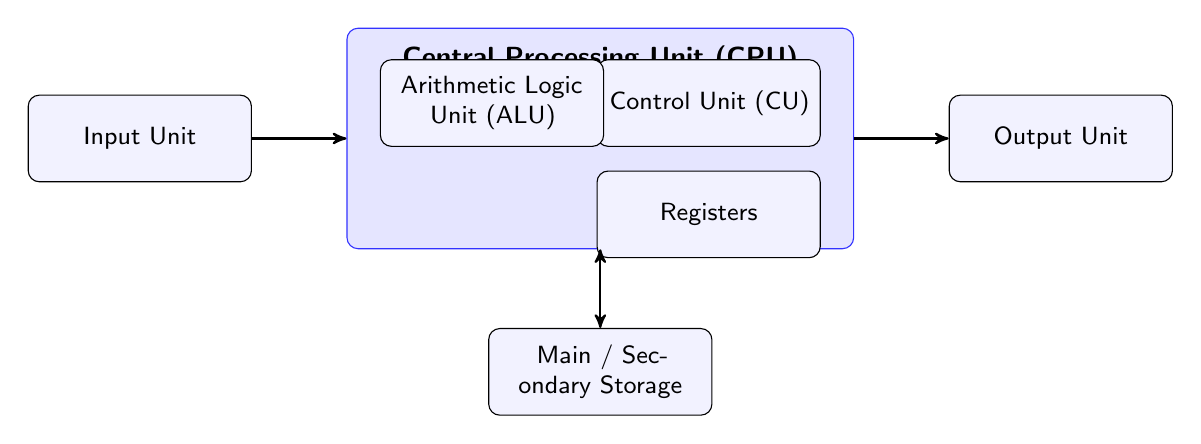
\begin{tikzpicture}[node distance=1.2cm, auto, >=stealth',
      block/.style={rectangle, draw, fill=blue!5, text width=2.6cm, text centered, rounded corners, minimum height=1.1cm, font=\small\sffamily},
      cpu/.style={rectangle, draw=blue!80, fill=blue!10, text width=6.2cm, text centered, rounded corners, minimum height=2.8cm, font=\small\sffamily}]
      
      \node [block] (input) {Input Unit};
      \node [cpu, right=1.2cm of input] (cpu) {};
      \node [font=\bfseries\sffamily, below=0.1cm of cpu.north] {Central Processing Unit (CPU)};
      \node [block, below left=0.4cm and -2.8cm of cpu.north] (cu) {Control Unit (CU)};
      \node [block, below right=0.4cm and -2.8cm of cpu.north] (alu) {Arithmetic Logic Unit (ALU)};
      \node [block, below=0.3cm of cu] (reg) {Registers};
      \node [block, right=1.2cm of cpu] (output) {Output Unit};
      \node [block, below=1.0cm of cpu] (memory) {Main / Secondary Storage};

      \draw[->, thick] (input) -- (cpu);
      \draw[->, thick] (cpu) -- (output);
      \draw[<->, thick] (cpu) -- (memory);
    \end{tikzpicture}
    \end{center}

  \item What is not correct regarding positional number systems?
    \begin{parts}
      \item The maximum value of a single digit is always equal to one less than the value of the base
      \item The value of each digit is determined by the digit itself
      \item Each symbol represents the same value regardless of its position in the number
      \item The value of each digit is determined by the base of the number system
    \end{parts}

  \item $(952)_{10} = ?_8$
    \begin{parts}
      \item 167
      \item 1670
      \item 761
      \item 7610
    \end{parts}

  \item What does `bit' stands for in computer terms?
    \begin{parts}
      \item Binary information term
      \item Binary digit
      \item Binary tree
      \item All of the above
    \end{parts}

  \item Registers are part of:
    \begin{parts}
      \item main memory
      \item secondary memory
      \item CPU
      \item ALU
    \end{parts}

  \item Megabyte (MB) is equal to:
    \begin{parts}
      \item $32\ (2^5)$ bytes
      \item $1024\ (2^{10})$ bytes
      \item $1,048,576\ (2^{20})$ bytes
      \item $1,073,741,824\ (2^{30})$ bytes
    \end{parts}
\end{parts}

\bigskip

\noindent \textbf{Question 2.}

\begin{parts}
  \item (i) Find the complement of $6_8$.\\[2pt]
        (ii) Subtract 5610 from 9210 using complementary method.\pts{7}
  \item Discuss different types of ROMs in detail.\pts{7}
\end{parts}

\bigskip

\noindent \textbf{Question 3.}

\begin{parts}
  \item Explain classification of commonly used secondary storage devices.\pts{7}
  \item How do we define magnetic tape storage capacity? What is the storage capacity of a magnetic tape if the tape density is 800 bpi and tape length is 600 feet?\pts{7}
\end{parts}

\bigskip

\noindent \textbf{Question 4.}

\begin{parts}
  \item What do you understand about the storage capacity of a magnetic disk system?\pts{7}
  \item Write in detail on which parameters magnetic disk access time depends upon.\pts{7}
\end{parts}

\bigskip

\noindent \textbf{Question 5.}

\begin{parts}
  \item Explain (i) relationship between hardware and software (ii) difference between software and Program.\pts{7}
  \item What do you understand about Database Management Systems (DBMS)? How is it different from file-oriented approach of organizing data?\pts{7}
\end{parts}

\bigskip

\noindent \textbf{Question 6.}

\begin{parts}
  \item Explain software development steps in detail.\pts{7}
  \item Write the difference between (i) system software and application software (ii) compiler and interpreter.\pts{7}
\end{parts}

\bigskip

\noindent \textbf{Question 7.}

\begin{parts}
  \item What do you understand about low-level and high-level languages? Write their advantages and limitations.\pts{7}
  \item What is the purpose of an operating system? Explain multiprogramming and multiprocessing techniques in detail.\pts{7}
\end{parts}

\vfill\rule{\linewidth}{0.4pt}
\end{document}
